\documentclass[11pt]{article}
%\usepackage{garamondx}
\usepackage[a4paper, total={210mm,297mm}, left=20mm, right=20mm, top=20mm, bottom=20mm]{geometry}
\usepackage{setspace}
\onehalfspacing
\usepackage{booktabs}
\usepackage{graphicx,amsmath,amssymb,amsfonts}
\usepackage{epsfig,lscape}
\usepackage{multicol,multirow,slashbox,color}
\usepackage{lifecon}
\usepackage[makeroom]{cancel}
\usepackage{tabulary,booktabs}
\usepackage{amsmath}
\usepackage{tikz}
\usepackage{mathtools}
\usetikzlibrary{calc,positioning}
\usetikzlibrary{arrows}
\def\tic{\tikz\fill[scale=0.6,red](0,.35) -- (.25,0) -- (1,.7) -- (.25,.15) -- cycle;} 
\usepackage{enumerate}
\usetikzlibrary{arrows,automata}
\pagenumbering{arabic}
\usepackage{fancyhdr,lastpage}
\pagestyle{fancy}
\fancyfoot[C]{Page \thepage\ of \pageref{LastPage}}
\renewcommand\headrulewidth{0in}
%\rhead{\bfseries{W1-2-60-1-6}}
%\lhead{\bfseries{STA 2191/ STA 2121}}
\usepackage{answers}
\newcommand{\sh}{\emph{shs }}
\newenvironment{problem}[1]{\begin{trivlist}\item \textbf{#1}. %
		\renewcommand{\Currentlabel}{#1}}{\end{trivlist}}
\Newassociation{solution}{Soln}{solutions}
\renewenvironment{Soln}[1]{\begin{trivlist}\item
		\textbf{#1}.}{\end{trivlist}}
\renewcommand{\mark}[1]{\hspace*{\fill}[{{#1}\:}{mark}]}
\renewcommand{\marks}[1]{\hspace*{\fill}[{{#1}\:}{marks}]}
\usepackage{pdfpages}
\usepackage{advdate}

\begin{document}
	\begin{figure}[h]
		\vspace{1cm}
		\centering
		
\includegraphics[width=0.2\textwidth]{logo}
	\end{figure}
\vspace{-0.1cm}
	\begin{center}
		\textbf{UNIVERSITY EXAMINATIONS 2024/2025\\
		YEAR 1 SEMESTER II EXAMINATION FOR THE DEGREE OF BACHELOR OF SCIENCE IN SPECIFY THE DEGREE}
	
	
	
	\end{center}
	\begin{center}
		\textbf{SPS 0001: SAMPLE EXAMINATION}
	\end{center}
	%\large
	\textbf{DATE: MONDAY $15^{TH}$ DECEMBER 2024} \hfill \textbf{TIME: 8.30 am - 10.30 am}\\
	\noindent\makebox[\linewidth]{\rule{\textwidth}{1.5pt}}
	\emph{\textbf{INSTRUCTIONS TO CANDIDATES:}
		\begin{enumerate}
			\item Answer question ONE and any other TWO questions.
			\item Be neat and show all your workings
		\end{enumerate}}
		\noindent\makebox[\linewidth]{\rule{\textwidth}{1.5pt}}
		This paper consists of 5 printed pages.
		
		
		\newpage
	%	\begin{center} \underline{\textbf{QUESTION ONE (30 MARKS)}} \end{center}
		\Opensolutionfile{solutions}[ans]
			\begin{center}
			\textbf{\underline{QUESTION ONE: 30 MARKS}}
		\end{center}
\begin{enumerate}
\item\begin{enumerate}
	\item Let $ A  = \begin{bmatrix}1 & 3\\
	4 & 5\end{bmatrix}$ find the characteristic polynomial of A. \marks{3}
   \item Let $F:\mathbb{R}^{2} \rightarrow \mathbb{R}^{2}$ be defined by $F(x,y) = (4x + 5y, 2x-y)$ and the following basis of $\mathbb{R}^{2}:E = \{e_{1}, e_{2}\} = \{(1,0), (0,1)\}$ and $S = \{u_{1},u_{2}\}= \{(1,2),(2,3)\}$. Find the matrix A representing F relative to the basis E. \marks{4}
   \item The center of a group $z(a) = \{X\in G|x*g = g*x, \forall g\in G\}$ prove that $z(a)$ is a subgroup. \marks{6}
   \item Let X be a topological space, show that the classes of closed subsets of $X$ possess the following properties:
   \begin{enumerate}[(i)]
   	\item $X$ and $\emptyset$ are closed sets. \mark{1}
   	\item The intersection of any closed set is closed. \marks{3}
   	\item The finite union of closed sets is closed. \marks{3}
   \end{enumerate}
\item Let $A = \{4,2,6,1\}$ and $B = \{a,2,c,5,4\}$ evaluate
\begin{enumerate}[(i)]
	\item $B-A$ \mark{1}
	\item $A \cap B$ \mark{1}
	\item $|A\cup B|$ \mark{1}
\end{enumerate}
\item From the following data estimate the value of $$\int_{1}^{5} \log x dx$$
Using Simpson's $\frac{1}{3}$ rule
\begin{table}[h!]
	\centering
	\begin{tabular}{|l|l|l|l|l|l|l|l|l|}
		\hline
		$x$          & 1.0   & 1.5    & 2.0    & 2.5    & 3.0    & 4.0    & 4.5    & 5.0    \\ \hline
		$Y = \log x$ & 0.000 & 0.4055 & 0.6931 & 0.9163 & 1.0986 & 1.3865 & 1.1041 & 1.6099 \\ \hline
	\end{tabular}
\end{table} \marks{5}
\item Solve the system of equation below by use of Gauss elimination method
with partial pivoting.\marks{5}
\begin{align*}
	x + y + z =7\\
	3x + 3y + 4z = 24\\
	2x + y + 3z = 16
\end{align*}


\end{enumerate}
%\newpage
\begin{center} \underline{\textbf{QUESTION TWO: 20 MARKS}} \end{center}
\item\begin{enumerate}
	\item A solid cylinder of 10cm diameter and 40 cm long consists of two parts made of different materials. The first part of the base is 1.0cm long and of specific gravity = 6.0. The other part of the cylinder is made of the material having a specific gravity of 0.6 as shown in Figure 1. Determine if it can float vertically in water. \marks{10}
	\begin{figure}[h!]
		\centering
		\label{figa1}
		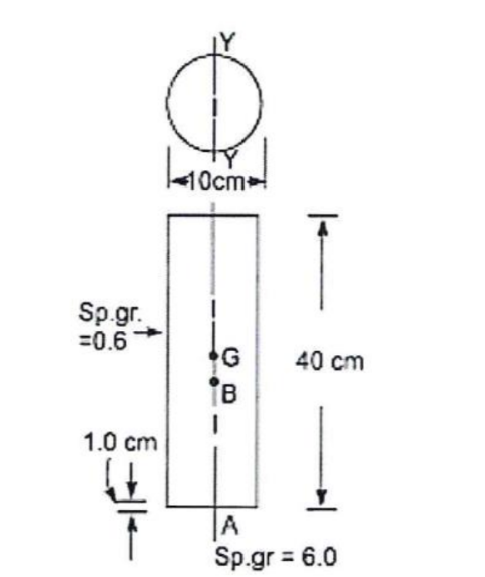
\includegraphics[width=80mm]{fm.png}
		\caption{Diagram for use}
	\end{figure}
\newpage
\item Evaluate the following limits
\begin{enumerate}[(i)]
	\item $\lim\limits_{x\rightarrow 0}$ $\dfrac{\sin x}{2x}$ \marks{3}
	\vspace{0.2cm}
	\item $\lim\limits_{x\rightarrow \infty}$ $\dfrac{8x^{3} - 9x -1}{-12x^{3}+1}$ \marks{3}
\end{enumerate}
\item For what values of the constant K is the function continuous for all values of $X$\marks{3}
\begin{equation*}
	f(x) = 
	\begin{dcases}
		KX + 5 &  X < 1  \\[1ex]
		x^{2}-3x + 4 & X \geq 1 
	\end{dcases}
\end{equation*}
\item Determine whether the series $\displaystyle{\sum_{n=1}^{\infty}}\frac{n}{n+1}$ converges or diverges. \marks{3}
\end{enumerate}
%\newpage
\begin{center} \underline{\textbf{QUESTION THREE: 20 MARKS}} \end{center}

\item\begin{enumerate}[(a)]
	\item In multiple regression, prove that the variance of $\hat{\beta_{0}}$ and $\hat{\beta_{1}}$
	$$V(\hat{\beta_{0}}) = \frac{\uparrow \sigma^{2}\displaystyle{\sum_{i=1}^{n}}x_{i}^{2}}{\displaystyle{\sum_{i=1}^{n}}(x_{i}-\bar{x})^{2}} \enspace and \enspace V(\hat{\beta_{1}}) = \frac{\sigma^{2}}{\displaystyle{\sum_{i=1}^{n}}(x_{i}-\bar{x})^{2}}$$ \marks{7}
	\item Assuming the factor ANOVA model $y_{ij} = \mu + t_{i} + e_{ij}$ where $e_{ij} \sim N(0,\sigma^{2})$
	\begin{enumerate}[(i)]
		\item Obtain the estimate $u_{1},t_{1}, t_{2}, t_{3}$ and $t_{4}$ of the factor level means. \marks{5}
		\item Test the hypothesis that the four types of fertilizers have the same response means
		against the alternative that the factor levels are not equal and construct the
		ANOVA.\marks{8}
	\end{enumerate}
\end{enumerate}

\begin{center} \underline{\textbf{QUESTION FOUR: 20 MARKS}} \end{center}
\item\begin{enumerate}[(a)]
	\item Write an R program that perform the following integrals. \marks{5}
	$$\int_{0}^{1} \int_{0}^{2} \int_{1}^{3} \frac{1}{150} (2x_{1}+ x_{2} + x_{3}^{2})dx$$
	\item Write an R Code to give the following output. \textbf{NB: Use for loop}\marks{5}
	\begin{verbatim}
		1*1 = 1
		3*3 = 9
		5*5 = 25
		7*7 = 49
		9*9 = 81
		11*11 = 121
		13*13 = 169
		15*15 = 225
	\end{verbatim}
\item Interpret the following multiple linear regression output. \marks{10}
\begin{verbatim}
	Call:
	lm(formula = Y ~ X1 + X2)
	
	Residuals:
	Min      1Q  Median      3Q     Max 
	-1.4568 -0.4870 -0.1646  0.8023  1.1672 
	
	Coefficients:
	Estimate Std. Error t value Pr(>|t|)  
	(Intercept)  -0.1123     0.4035  -0.278   0.7887  
	X1            0.4580     0.5331   0.859   0.4187  
	X2           -0.4837     0.2475  -1.954   0.0916 .
	---
	Signif. codes:  0 ‘***’ 0.001 ‘**’ 0.01 ‘*’ 0.05 ‘.’ 0.1 ‘ ’ 1
	
	Residual standard error: 1.051 on 7 degrees of freedom
	Multiple R-squared:    0.4,	Adjusted R-squared:  0.2285 
	F-statistic: 2.333 on 2 and 7 DF,  p-value: 0.1673
\end{verbatim}
\end{enumerate}
\begin{center} \underline{\textbf{QUESTION FIVE: 20 MARKS}} \end{center}

%\newpage
\item\begin{enumerate}[(a)]
	\item Use Taylor's series to show that if $h$ is small then
	$$\tan^{-1}(x+h)\cong \tan^{-1}x + \frac{h}{1+x^{2}} - \frac{xh^{2}}{(1+x^2)^{2}} $$ \marks{5}
	\item Given that $f(x,y) = tan^{-1}(\dfrac{y}{x})$ show that $\dfrac{\partial^{2}f}{\partial x \partial y} = \dfrac{\partial^{2} f}{\partial y \partial x}$ \marks{6}
	\item If $z = x^{2} + y^{2}$ where $x = r\cos \theta$ and $y = r \sin 2\theta $ find $\frac{\partial z}{\partial r}$ and $\frac{\partial z}{\partial \theta}$ \marks{10}
\end{enumerate}
\end{enumerate}
%\Closesolutionfile{solutions}
\begin{center}
THE END
\par\end{center}
%\newpage
%\setcounter{page}{1}
%\begin{center}
%\underline{SPM 2441: REGRESSION MODELLING SOLUTIONS}
%\par\end{center}
%\Readsolutionfile{solutions}
\end{document}